\documentclass[10pt,journal]{IEEEtran}

\usepackage[utf8]{inputenc}
\usepackage[T1]{fontenc}
\usepackage{amsmath,amssymb,amsfonts,amsthm}
\usepackage{graphicx}
\usepackage{booktabs}
\usepackage{cite}
\usepackage{url}
\usepackage{microtype}
\usepackage{tabularx}

\graphicspath{{figuras/}}

\newtheorem{remark}{Remark}

\begin{document}

\title{Contract Resale Flexibility Under Market and Regulatory Constraints in the Brazilian Electricity Market}

\author{Marcelo~Albuquerque~Heluy,%
        ~Fernando~Bezerra~Chagas,%
        ~Jo\~ao~Guilherme~Raposo~Lobato,%
        ~and~Francisco~Glaubos~Nunes~Cl\'imaco%
\thanks{F. G. N. Cl\'imaco is with the Department of Computer Science, Federal University of Maranh\~ao (UFMA), S\~ao Lu\'is, MA 65080-805, Brazil (e-mail: francisco.glaubos@ufma.br).}%
\thanks{F. B. Chagas is with the Federal Institute of Maranh\~ao (IFMA), Imperatriz Campus, and the Graduate Program in Computing, Fluminense Federal University (UFF), Brazil (e-mail: fernando.chags@ifma.edu.br).}%
\thanks{M. A. Heluy is with the Federal University of Maranh\~ao (UFMA), Brazil (e-mail: marcelo.ag@discente.ufma.br).}%
\thanks{J. G. R. Lobato is with the Federal University of Maranh\~ao (UFMA), Brazil (e-mail: joao.lobat@discente.ufma.br).}%
\thanks{Manuscript received November 2026.}}

\markboth{IEEE Transactions on Energy Markets, Policy and Regulation,~Vol.~X, No.~Y, 2026}%
{Heluy \MakeLowercase{\textit{et al.}}: Contract Resale Flexibility Under Market and Regulatory Constraints}

\IEEEtitleabstractindextext{%
\begin{abstract}
Standard electricity retail portfolio models prohibit secondary forward contract resale, locking commercializers into buy-and-hold positions despite demand churn and spot volatility. We formulate a monthly multistage stochastic linear program calibrated on Brazilian Clearinghouse (CCEE) hourly spot prices (2021--2023) that integrates uniform block products, backed contract resale, Southeast/Northeast submarket balance, Mean--CVaR risk aversion, and Decree~5.163/2004 trailing 12-month backing penalties. Under joint price--demand scenario branching and competitive free-market retail margins, dynamic resale raises the in-sample Mean--CVaR objective across 10 paired seeds by $+3.98\%$ ($\text{R\$}\,0.75/\text{MWh}$, positive in all seeds) and sustains $96.5\%$ statutory backing compliance under the VR penalty versus $60.9\%$ breach incidence for static 95\% hedging. However, once out-of-sample evaluations eliminate own-tree forward execution through exogenous market forward curves, dynamic resale loses its advantage over passive benchmarks: in a 2024--2025 rolling backtest with flat load, the mean profit difference between resale and buy-and-hold ($-\text{R\$}\,0.273\,\text{M}$/mo., 95\% bootstrap CI $[-1.102, +0.325]\,\text{M}$/mo.) is statistically insignificant, while buy-and-hold exhibits lower profit dispersion ($\text{SD}\;\text{R\$}\,6.38\,\text{M}$ vs.\ $\text{R\$}\,8.81\,\text{M}$), milder monthly tail losses ($\mathrm{CVaR}_{0.05}^{\mathrm{profit}}\;-\text{R\$}\,0.76\,\text{M}$ vs.\ $-\text{R\$}\,2.64\,\text{M}$), smaller trailing 12-month backing deficits ($4.4$ vs.\ $58.7\,\text{GWh}$), and lower peak collateral ($\text{R\$}\,6.95\,\text{M}$ vs.\ $\text{R\$}\,12.57\,\text{M}$). Across 1,000 independent synthetic churn trajectories, resale likewise yields statistically insignificant mean differences ($+\text{R\$}\,0.46\,\text{M}$, CI $[-0.32, +1.24]\,\text{M}$) while trailing static hedging in tail protection. Scenario-tree misspecification and market forward divergence, rather than trading frictions alone, govern real-world dynamic hedging performance.
\end{abstract}

\begin{IEEEkeywords}
Electricity retail, Multistage stochastic programming, Forward contract resale, Conditional Value-at-Risk, Regulatory backing, Brazilian electricity market, DESSEM.
\end{IEEEkeywords}}

\maketitle
\IEEEdisplaynontitleabstractindextext
\IEEEpeerreviewmaketitle

\section{Introduction}

\IEEEPARstart{E}{lectricity} commercializers act as intermediaries between wholesale generation and end-use consumers, procuring multi-horizon forward contracts to hedge retail obligations while settling physical imbalances in the short-term pool~\cite{Conejo2010,Hatami2009,Carrion2007,EPSR2026}. In Brazil's Free Contracting Environment (\textit{Ambiente de Contrata\c{c}\~ao Livre}, ACL), two structural shifts have amplified retail risk since 2021: the deployment of hourly spot pricing via the DESSEM model~\cite{Santos2020,CCEE2024}, which revealed steep intra-day ramps and Northeast-to-Southeast locational decoupling, and Ordinance~50/GM/MME~\cite{PortariaMME50_2022}, which opened the ACL to all Group~A high-voltage consumers in January 2024 alongside the retail marketer regime (\textit{comercializador varejista})~\cite{ANEEL_REN1011_2022,ANEEL_REN1014_2022,ANEEL_REN1081_2023}, intensifying client churn.

Conventional retail optimization models often assume two stages or prohibit secondary contract liquidation~\cite{Carrion2007,OumOren2010,Mansini2007,Kettunen2010}. Under a rigid buy-and-hold policy, demand drops leave retailers over-contracted and exposed to depressed spot prices, while under-contracting violates statutory backing obligations under Decree~5.163/2004~\cite{Decreto5163_2004}. This paper addresses the research question: \textit{what is the quantitative economic and regulatory value of backed forward contract resale for electricity commercializers under spot volatility, demand churn, and statutory backing rules, both in-sample and out-of-sample against exogenous market forward curves?}

\subsection{Key Contributions}
We develop a monthly multistage stochastic linear program (MSLP) calibrated from CCEE hourly spot series, yielding three contributions:
\begin{enumerate}
    \item \textit{Brazilian Market and Regulatory Formulation:} Across an 8-quarter horizon (24 months), the model integrates Southeast/Midwest (SE) and Northeast (NE) submarket balance, statutory ANEEL spot limits~\cite{ANEEL_REH2828_2020,ANEEL_REH2994_2021,ANEEL_REH3167_2022,ANEEL_REH3304_2023,ANEEL_Despacho3625_2024}, systemic reserve charges (ESS/EER, \textit{Encargos de Servi\c{c}os do Sistema} and \textit{Energia de Reserva}), uniform monthly/quarterly/semiannual block delivery, backed resale constraints, and Decree~5.163/2004 trailing 12-month coverage penalties (ANEEL REN~1.090/2024)~\cite{ANEEL_REN1090_2024,ANEEL_Despacho3176_2024} alongside prudential coverage floors.
    \item \textit{Joint Price--Demand Tree, Paired Benchmarks, and Extensions:} Using joint standardized Principal Component Analysis (PCA) bisection over SE/NE prices and demand, we assess resale performance using 10-seed paired in-sample and Kaut--Wallace out-of-sample evaluations, quantify the Value of Multistage Recourse ($\mathrm{VMR}$) against a two-stage Mean--CVaR benchmark, separate constant vs.\ maturity-decaying risk premia, and test extensions for hourly load modulation and monthly $\text{NE}\to\text{SE}$ Financial Transmission Rights (FTRs).
    \item \textit{Exogenous-Curve Historical and 1,000-Path OOS Validation:} Evaluating rolling policies against exogenous market forward curves (seasonal log-AR(1) in 2024--2025 and exact analytical conditional expectations over 1,000 non-Markovian synthetic trajectories, plus consumer-price-deflated 2001--2023 trees using Brazil's official IPCA index), we demonstrate that eliminating own-tree forward execution alters out-of-sample rankings and shows when buy-and-hold and static hedges outperform rolling reoptimization.
\end{enumerate}

\section{Related Literature}
\label{sec:lit}

Risk-constrained electricity portfolio optimization routinely adopts Conditional Value-at-Risk (CVaR) for its coherence and linear programming tractability~\cite{Conejo2010,BirgeLouveaux2011,RockafellarUryasev2000,RockafellarUryasev2002,Mansini2007}. Classical retail formulations focus on two-stage forward procurement and tariff setting~\cite{Carrion2007,Hatami2009}, while Oum and Oren~\cite{OumOren2010} derive optimal static hedging policies under correlated price and volumetric demand risk. Multistage stochastic programming generalizes these frameworks to sequential recourse~\cite{BirgeLouveaux2011,PflugPichler2014,Shapiro2021}, building on multi-period electricity hedging~\cite{Fleten2002}, moment matching~\cite{HoylandWallace2001}, scenario reduction~\cite{HeitschRomisch2003,HeitschRomisch2009}, and empirical comparisons of scenario-generation methods and out-of-sample stability~\cite{KautWallace2007,Lohndorf2016}.

In retail portfolios, Kettunen et al.~\cite{Kettunen2010} model multistage CVaR procurement but omit explicit backed forward resale under bilateral bid-ask spreads. In the Brazilian market, Santos et al.~\cite{Santos2020} document the DESSEM hourly pricing architecture, while risk-averse Stochastic Dual Dynamic Programming (SDDP) with nested CVaR has been developed for hydrothermal dispatch planning (NEWAVE)~\cite{PhilpottMatos2012,Shapiro2013} and generator contracting~\cite{Street2009,Fanzeres2015,EPSR2026}. Unlike nested CVaR, terminal Mean--CVaR lacks dynamic time consistency across stages~\cite{Shapiro2009,Shapiro2021}; rather than adopting multi-stage nested risk measures that complicate comparative two-stage and static benchmarks, we follow standard retail practice with terminal Mean--CVaR and audit dynamic consistency explicitly via rolling-horizon out-of-sample reoptimization.

\section{Market Architecture and Regulatory Framework}
\label{sec:market}

The Brazilian power sector comprises the Regulated Contracting Environment (ACR) and the bilateral ACL~\cite{CCEE2024}, where CCEE settles metered imbalances against registered contracts at the Difference Settlement Price (PLD). Since January 1, 2021, DESSEM computes 24 hourly PLDs per day across four submarkets, producing pronounced NE-to-SE locational divergence whenever NE wind and solar generation saturates inter-regional transmission corridors~\cite{Santos2020,CCEE2024}. As shown by the empirical complementary cumulative distribution function (CCDF) in Fig.~\ref{fig:pld_spread}, the mean hourly spread $\text{PLD}_{\text{SE}} - \text{PLD}_{\text{NE}}$ rose from $\text{R\$}\,3.70/\text{MWh}$ in 2021--2023 to $\text{R\$}\,28.30/\text{MWh}$ in 2024--2025, with hourly spikes reaching $\text{R\$}\,589.18/\text{MWh}$ (calibration) and $\text{R\$}\,572.63/\text{MWh}$ (testing).

\begin{figure}[t]
\centering
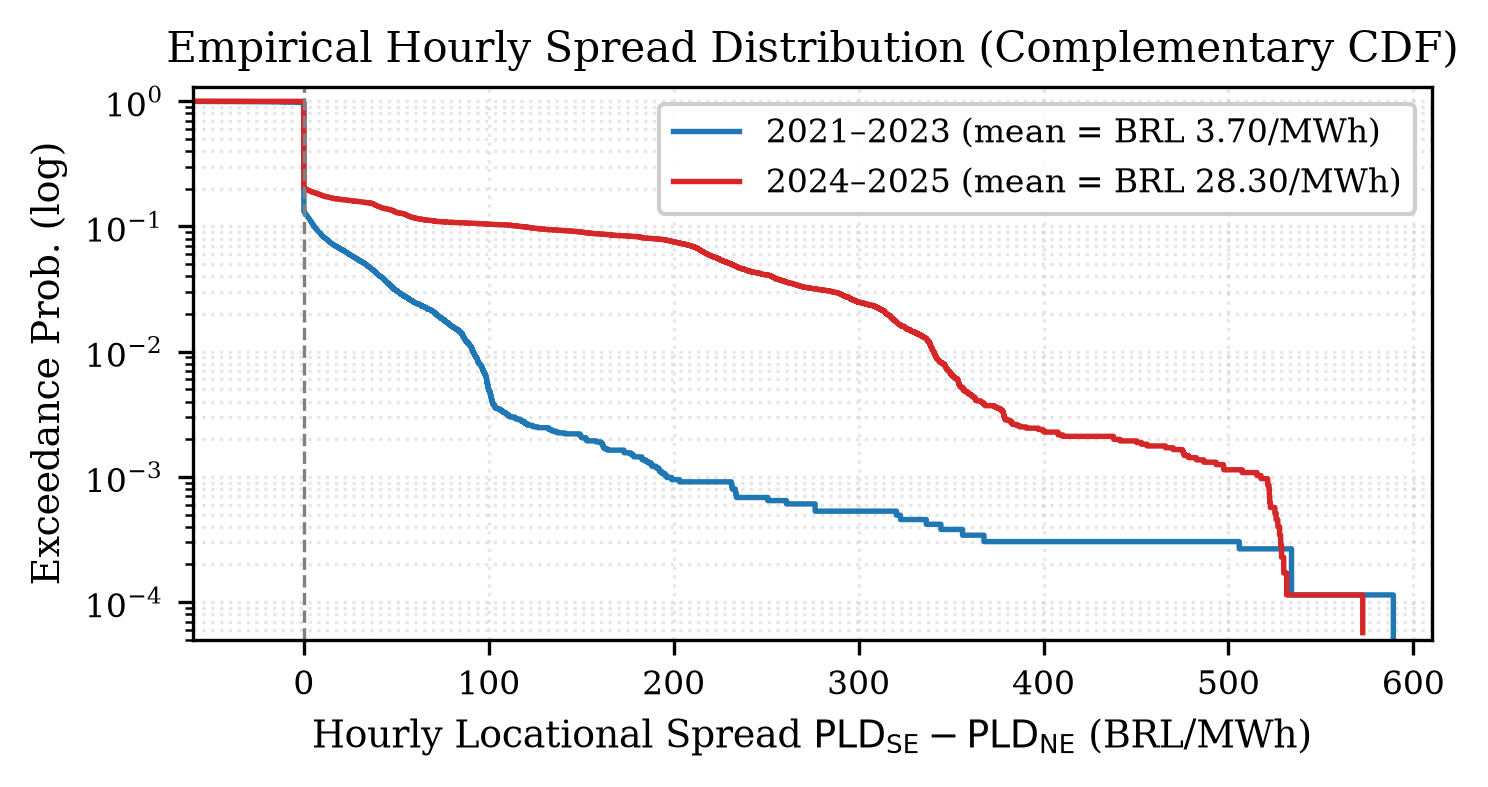
\includegraphics[width=\columnwidth]{fig_tempr_pld_spread.png}
\caption{Empirical complementary CDF (log scale exceedance probability) of the hourly locational spread $\mathrm{PLD}_{\mathrm{SE}} - \mathrm{PLD}_{\mathrm{NE}}$ from official CCEE data during calibration (2021--2023) and testing (2024--2025).}
\label{fig:pld_spread}
\end{figure}

To contain credit risk, ANEEL updates annual statutory PLD bounds every December, distinguishing monthly structural ceilings from hourly ceilings (Table~\ref{tab:pld_bounds}). These asymmetric limits truncate downside prices near run-of-river hydro operating costs while allowing upside spikes up to $\text{R\$}\,1,542.23/\text{MWh}$ in 2025.

Beyond spot settlement, Decree~5.163/2004~\cite{Decreto5163_2004} requires sellers to hold 100\% physical or contractual backing for sales and buyers to maintain 100\% contractual coverage for realized consumption, audited monthly by CCEE over a trailing 12-month moving window. ANEEL REN~1.090/2024~\cite{ANEEL_REN1090_2024} (effective January 2025) values penalties at the Annual Reference Value (VR), replacing the higher of VR and PLD and thus reducing penalties when PLD exceeds VR. CCEE reports the 2025 VR as $\text{R\$}\,231.47/\text{MWh}$~\cite{CCEE_VR2025}. In addition, Ordinance~50/GM/MME~\cite{PortariaMME50_2022} and ANEEL RENs~1.011/2022, 1.014/2022, and 1.081/2023~\cite{ANEEL_REN1011_2022,ANEEL_REN1014_2022,ANEEL_REN1081_2023} require consumers below $500\,\text{kW}$ to be represented by Type~1 retail marketers (\textit{comercializador varejista}) subject to minimum net equity and CCEE short-term financial collateral calls. Retail consumers also bear non-commodity System Service and Reserve Energy Charges (ESS/EER)~\cite{CCEE2024}, modeled in the baseline via a deterministic levy $\tau_{\text{reg}} = \text{R\$}\,15.00/\text{MWh}$. Bilateral forward trading occurs over-the-counter on electronic trading venues such as the \textit{Balc\~ao Brasileiro de Comercializa\c{c}\~ao de Energia} (BBCE, which operates as an OTC order-matching platform rather than a central counterparty clearinghouse) and via centrally cleared contracts on B3 in standardized monthly ($M$), quarterly ($T$), and semiannual ($S$) blocks, where secondary liquidation incurs a one-way half-spread $\sigma$.

\begin{table}[t]
\centering
\caption{Official ANEEL Statutory PLD Boundaries (2021--2025, R\$/MWh).}
\label{tab:pld_bounds}
\scriptsize
\setlength{\tabcolsep}{4pt}
\begin{tabular}{ccccc}
\toprule
Year & ANEEL Act & Floor & Struct.\ Ceiling & Hourly Ceiling \\
\midrule
2021 & REH 2.828/2020~\cite{ANEEL_REH2828_2020} & 49.77 & 583.88 & 1,197.87 \\
2022 & REH 2.994/2021~\cite{ANEEL_REH2994_2021} & 55.70 & 646.58 & 1,326.50 \\
2023 & REH 3.167/2022~\cite{ANEEL_REH3167_2022} & 69.04 & 684.73 & 1,404.77 \\
2024 & REH 3.304/2023~\cite{ANEEL_REH3304_2023} & 61.07 & 716.80 & 1,470.57 \\
2025 & Desp.\ 3.625/2024~\cite{ANEEL_Despacho3625_2024} & 58.60 & 751.73 & 1,542.23 \\
\bottomrule
\end{tabular}
\end{table}

\section{Mathematical Formulation}
\label{sec:math}

Uncertainty is modeled on a filtered probability space $(\Omega, \mathcal{F}, \{\mathcal{F}_t\}_{t=0}^{T-1}, \mathbb{P})$ discretized as a scenario tree $\mathcal{N}$ with stages $t \in \mathcal{T} = \{0, \dots, T-1\}$, root $\nu = 0$, parent $a(\nu)$, ancestor path $\mathcal{P}(\nu)$, unconditional node probabilities $\pi_\nu$, and terminal leaves $\mathcal{L} \subset \mathcal{N}$ ($\sum_{\ell \in \mathcal{L}} \pi_\ell = 1$)~\cite{BirgeLouveaux2011,Shapiro2021}. Non-anticipativity holds by indexing all decisions by $\nu \in \mathcal{N}$; complete nomenclature appears in Supplementary Material Table~S1.

\subsection{Block Products, State Transitions, and Physical Bounds}
Let $\mathcal{M}(\nu)$ denote the delivery months governed by node $\nu$, $s \in \mathcal{S} = \{\text{SE}, \text{NE}\}$ the submarkets, and $k \in \mathcal{K} = \{M, T, S\}$ the forward tenors with delivery calendar sets $\mathcal{B}_{k,p}$ ($|\mathcal{B}_{M,p}|=1$, $|\mathcal{B}_{T,p}|=3$, $|\mathcal{B}_{S,p}|=6$). A forward block $(k, p)$ is tradable at $\nu$ only if all delivery months exceed $\max \mathcal{M}(\nu)$:
\begin{equation}
\mathcal{P}_k(\nu) = \left\{ p : \min(\mathcal{B}_{k,p}) \ge \max \mathcal{M}(\nu) + 1 \right\}.
\label{eq:eligibility}
\end{equation}
Condition~\eqref{eq:eligibility} implies that when initial inherited positions are zero ($q_{a(0),s,n} = 0$), the first quarter ($n \in \{0,1,2\}$) cannot be hedged in single-shot runs, contributing to unhedged tail exposure at $\lambda = 0$. Indexing purchase $x^+_{\nu,s,k,p} \ge 0$ and resale $x^-_{\nu,s,k,p} \ge 0$ (MWmed) by block $(k,p)$ enforces uniform capacity across all $n \in \mathcal{B}_{k,p}$. With indicator $\delta_{k,p,n} = \mathbf{1}_{\{n \in \mathcal{B}_{k,p}\}}$, the cumulative net forward position $q_{\nu,s,n}$ evolves for $n \ge \min \mathcal{M}(\nu)$ as:
\begin{equation}
q_{\nu,s,n} = q_{a(\nu),s,n} + \sum_{k \in \mathcal{K}} \sum_{p \in \mathcal{P}_k(\nu)} \delta_{k,p,n} \left( x^+_{\nu,s,k,p} - x^-_{\nu,s,k,p} \right),
\label{eq:state_q}
\end{equation}
where $q_{a(0),s,n}$ equals zero in single-shot runs or inherited positions in rolling backtests. Prudential headroom and optional minimum coverage floors $\underline{c} \in \{0, 1.0\}$ (applied over contractable months $n \ge \max\mathcal{M}(0)+1$) bound $q_{\nu,s,n}$ relative to base and peak scenario demand $D^{\max}_{s,n} = \max_{\mu \in \mathcal{N}} D_{\mu,s,n}$:
\begin{equation}
\underline{c}\,D^{\text{base}}_{s,n}\le q_{\nu,s,n}\le\kappa\,D^{\max}_{s,n},\;\forall \nu\in\mathcal{N},\,s\in\mathcal{S},\,n\ge\min\mathcal{M}(\nu),
\label{eq:physical_bound}
\end{equation}
with $\kappa = 1.0$ and $\underline{c} = 0$ in the baseline (the upper bound is active in 38.8\% of SE and 19.7\% of NE node-months at $\lambda = 0.50$).

\subsection{Physical Balance, Resale Backing, and Decree~5.163/2004}
For each month $m \in \mathcal{M}(\nu)$, spot surplus $y^+_{\nu,s,m} \ge 0$ and deficit $y^-_{\nu,s,m} \ge 0$ satisfy:
\begin{equation}
y^+_{\nu,s,m} - y^-_{\nu,s,m} = E_{\nu,s,m} - D_{\nu,s,m} + q_{\nu,s,m},
\label{eq:phys_balance}
\end{equation}
where $D_{\nu,s,m} = D^{\text{base}}_{s,m} \theta_{\nu,m}$ is client load (abstracting from retail contract take-or-pay flexibility bands, which represent a relevant extension for future work) and $E_{\nu,s,m} = 0$ is self-generation in the pure-retailer baseline. To prohibit naked short selling, cumulative resales along $\mathcal{P}(\nu)$ cannot exceed inherited plus cumulative purchases and $E_{\nu,s,n}$ for all $n \ge \min \mathcal{M}(\nu)$:
\begin{multline}
\sum_{\mu \in \mathcal{P}(\nu)} \sum_{k \in \mathcal{K}} \sum_{p \in \mathcal{P}_k(\mu)} \delta_{k,p,n} x^-_{\mu,s,k,p} \\
\le q_{a(0),s,n} + \sum_{\mu \in \mathcal{P}(\nu)} \sum_{k \in \mathcal{K}} \sum_{p \in \mathcal{P}_k(\mu)} \delta_{k,p,n} x^+_{\mu,s,k,p} + E_{\nu,s,n}.
\label{eq:resale_bound}
\end{multline}

\begin{remark}
When $E_{\nu,s,n} = 0$ and $\underline{c} = 0$,~\eqref{eq:state_q} and~\eqref{eq:resale_bound} are algebraically equivalent to $q_{\nu,s,n} \ge 0$ in~\eqref{eq:physical_bound}; hence~\eqref{eq:resale_bound} is redundant in the pure-retailer baseline ($E=0$) and is retained explicitly so the LP accommodates self-generation portfolios ($E_{\nu,s,m} > 0$) without reformulation. In the buy-and-hold benchmark (ME), secondary sales are capped at $E_{\nu,s,n}$, enforcing $x^- = 0$ when $E = 0$.
\end{remark}

To model Decree~5.163/2004~\cite{Decreto5163_2004} and ANEEL REN~1.090/2024~\cite{ANEEL_REN1090_2024} in Section~\ref{sec:reg_exp}, we introduce a trailing 12-month backing-deficit slack $d^{\text{las}}_{\nu,m} \ge 0$ over fully contractable windows ($m \ge 14$, spanning months $m-11$ to $m$ via the ancestor path $\nu_{k}$ governing month $k \in \mathcal{P}(\nu)$):
\begin{equation}
d^{\text{las}}_{\nu,m} \ge \frac{1}{12} \sum_{k=m-11}^{m} \sum_{s \in \mathcal{S}} \left( D_{\nu_k, s, k} - E_{\nu_k, s, k} - q_{\nu_k, s, k} \right),
\label{eq:lastro_12m}
\end{equation}
penalized in $C_\nu$ at $\pi_{\text{VR}} = \text{R\$}\,231.47/\text{MWh}$ via $-\sum_{m \in \mathcal{M}(\nu), m \ge 14} h_m \pi_{\text{VR}} d^{\text{las}}_{\nu,m}$ ($\pi_{\text{VR}} = 0$ in the unconstrained baseline). We also track ex-post the 95th percentile of peak two-month short spot exposure, $\max_{k} \sum_{m \in \{k, k+1\}, s} h_m \text{PLD}_{s,m} [D_{s,m} - q_{s,m}]^+$, as a proxy for CCEE financial collateral calls.

\subsection{Node-Conditional Forward Pricing and Risk Premia}
Let $h_m$ denote hours in month $m$ and $H_{k,p} = \sum_{n \in \mathcal{B}_{k,p}} h_n$. At node $\nu$, the tree-implied forward price of block $(k, p)$ is the hour-weighted conditional expectation of descendant spot prices $\text{PLD}_{s,n}$:
\begin{equation}
P^{\text{fwd}}_{\nu,s,k,p} = \frac{1}{H_{k,p}} \sum_{n \in \mathcal{B}_{k,p}} h_n \, \mathbb{E}\!\left[\text{PLD}_{s,n} \mid \nu\right] (1 + \psi_{\nu,k,p}),
\label{eq:pfwd}
\end{equation}
where $\psi_{\nu,k,p}$ is an optional risk premium ($\psi = 0$ in baseline; Section~\ref{sec:premio} compares constant $\psi_0 \in [-10\%, +10\%]$ against maturity-decaying $\psi_0 \tau_{\nu,k,p}$ with $\tau_{\nu,k,p} = \max(0, \bar{n}_{k,p} - \max \mathcal{M}(\nu))/(M-3) \in [0,1]$). Quotes apply half-spread $\sigma$ ($1.0\%$ base) scaled by tenor liquidity $\eta_k \in \{1.0, 0.8, 0.6\}$ for $\{M, T, S\}$:
\begin{equation}
P^+_{\nu,s,k,p} = P^{\text{fwd}}_{\nu,s,k,p} (1 + \eta_k \sigma), \quad P^-_{\nu,s,k,p} = P^{\text{fwd}}_{\nu,s,k,p} (1 - \eta_k \sigma).
\end{equation}
Analysis of 2023 empirical BBCE trading volumes (Supplementary Table~S11) confirms that while prompt monthly contracts ($M_0$--$M_{-2}$) hold the deepest near-term liquidity ($348.4$--$3,740.9\,\text{MWmed}$), quarterly blocks carry $3.6$--$9.4$ times larger depth than monthly contracts at forward horizons $L \ge 6$ months ($267.3$--$306.8$ vs.\ $28.4$--$85.2\,\text{MWmed}$), supporting narrower relative half-spreads ($\eta_S < \eta_T < \eta_M$) across tradable multi-month blocks beyond the excluded front quarter. When $\psi = 0$ and $\sigma > 0$, forward purchases carry negative expected return ($P^+ > \mathbb{E}[\text{PLD} \mid \nu]$), so under risk neutrality ($\lambda = 0$) optimal hedging is zero ($q^* = 0$) and $\text{ME-R} = \text{ME}$.

\subsection{Cash Flow, Mean--CVaR Objective, and Benchmarks}
At each node $\nu$, net cash flow $C_\nu = \Phi^{\text{cli}}_\nu + \Phi^{\text{fwd}}_\nu + \Phi^{\text{spot}}_\nu - \Phi^{\text{VR}}_\nu$ sums net retail revenues, forward trading cash flows, spot settlement, and any backing penalty:
\begin{align}
\Phi^{\text{cli}}_\nu &= \sum_{s \in \mathcal{S}} \sum_{m \in \mathcal{M}(\nu)} h_m \left( P^{\text{cli}} - \tau_{\text{reg}} \right) D_{\nu,s,m}, \\
\Phi^{\text{fwd}}_\nu &= \sum_{s \in \mathcal{S}} \sum_{k \in \mathcal{K}} \sum_{p \in \mathcal{P}_k(\nu)} H_{k,p} \nonumber \\
&\qquad \cdot \left( P^-_{\nu,s,k,p} x^-_{\nu,s,k,p} - P^+_{\nu,s,k,p} x^+_{\nu,s,k,p} \right), \\
\Phi^{\text{spot}}_\nu &= \sum_{s \in \mathcal{S}} \sum_{m \in \mathcal{M}(\nu)} h_m \text{PLD}_{\nu,s,m} \left( y^+_{\nu,s,m} - y^-_{\nu,s,m} \right).
\end{align}
To represent realistic competitive ACL retail margins rather than regulated captive tariffs, we calibrate the baseline sales tariff at $P^{\text{cli}} = \text{R\$}\,160.00/\text{MWh}$ (a gross margin of $\text{R\$}\,22.73/\text{MWh}$, or $16.56\%$, above the expected baseline spot plus $\tau_{\text{reg}} = \text{R\$}\,15.00/\text{MWh}$ cost of $\text{R\$}\,137.27/\text{MWh}$; Table~S10 reports sensitivity across $\text{R\$}\,150$--$260/\text{MWh}$). Leaf cumulative profit is $R_\ell = \sum_{\nu \in \mathcal{P}(\ell)} C_\nu$. Using Rockafellar--Uryasev linearization~\cite{RockafellarUryasev2000,RockafellarUryasev2002} with CVaR confidence $\beta = 0.95$, VaR threshold $\alpha$, shortfall slacks $u_\ell$, and risk-aversion weight $\lambda \in [0, 1)$, the LP solves:
\begin{equation}
\max_{\Xi} \quad (1 - \lambda) \sum_{\ell \in \mathcal{L}} \pi_\ell R_\ell - \lambda \left[ \alpha + \frac{1}{1 - \beta} \sum_{\ell \in \mathcal{L}} \pi_\ell u_\ell \right],
\label{eq:cvar_obj}
\end{equation}
subject to $u_\ell \ge -R_\ell - \alpha$, $u_\ell \ge 0$, \eqref{eq:state_q}--\eqref{eq:lastro_12m}, and $x^+, x^-, y^+, y^- \ge 0$. Tail risk is reported uniformly as expected 5\% worst-case profit $\mathrm{CVaR}_{0.05}^{\mathrm{profit}}(R) \triangleq -\mathrm{CVaR}_{0.95}^{\mathrm{loss}}(-R)$; at $\lambda = 0$, $\mathrm{CVaR}_{0.05}^{\mathrm{profit}}$ is computed ex-post on the risk-neutral optimal profit distribution $R^*$.

We benchmark \textit{ME-R} (multistage with resale) and \textit{ME} (buy-and-hold, $x^- = 0$) against three references: (i) \textit{2S} (a two-stage Mean--CVaR LP where root-stage forward contracts are chosen at $t=0$ and held rigidly across all scenarios without $t \ge 1$ forward recourse, allowing only physical spot settlement $y^+, y^-$ and CVaR slacks $u_\ell$ to adapt); (ii) \textit{HEUR} (passive 95\% root-stage monthly hedge of $D^{\text{base}}_{s,n}$); and (iii) \textit{Unhedged (DET)} (the deterministic expected-value LP, which buys zero forwards under $\sigma > 0$ and $\psi = 0$ and therefore executes zero hedges in both in-sample and rolling tests). Because terminal Mean--CVaR in~\eqref{eq:cvar_obj} is not time-consistent across stages~\cite{Shapiro2009,Shapiro2021}, rolling backtests in Section~\ref{sec:backtest} re-solve an updated conditional problem each quarter.

\subsection{Structural Extensions (Hourly Modulation and FTRs)}
\label{sec:ext_math}
To test intra-month shape and regional basis risks in Section~\ref{sec:ext_res}, we evaluate two extensions (Supplementary Section~S4): (i) \textit{hourly load modulation} adds $-(\gamma_{s,m} - 1)\,\text{PLD}_{\nu,s,m}\,D_{\nu,s,m}\,h_m$ to $\Phi^{\text{spot}}_\nu$, where $\gamma_{s,m} = \frac{\sum_{h \in m} \text{PLD}^{\text{h}}_{s,h} D^{\text{h}}_{s,h}}{\text{PLD}_{s,m} \sum_{h \in m} D^{\text{h}}_{s,h}}$ is the capture ratio of hourly profile $D^{\text{h}}_{s,h}$ relative to flat forwards; and (ii) \textit{cross-submarket $\text{NE}\to\text{SE}$ contracting} permits $q^{\text{cross}}_{\nu,n} \ge 0$ purchased at NE forwards to serve SE load ($q_{\nu,\text{SE},n} + q^{\text{cross}}_{\nu,n} \le \kappa D^{\max}_{\text{SE},n}$) alongside an optional monthly FTR $0 \le q^{\text{FTR}}_{\nu,n} \le q^{\text{cross}}_{\nu,n}$ priced at $\mathbb{E}[\max(0, \text{PLD}_{\text{SE},n} - \text{PLD}_{\text{NE},n}) \mid \nu] + c_{\text{FTR}}$.

\section{Data Calibration and Scenario Tree}
\label{sec:data}

\subsection{Empirical Dataset and Chronological Partitioning}
Official CCEE hourly PLD series for SE and NE are partitioned chronologically without look-ahead into a calibration pool (2021--2023, 26,280 hours/submarket) and an out-of-sample test set (2024--2025, 17,544 hours/submarket). Because CCEE transitioned from weekly load-level pricing to hourly DESSEM clearing on January 1, 2021~\cite{Santos2020}, any longer calibration stretching back to 2001--2020 blends distinct price-formation regimes and statutory caps and must therefore account for consumer price inflation.

\subsection{Reproducible Scenario Tree Construction}
The 24-month horizon comprises $T=8$ quarterly stages generated from a random seed via four deterministic steps:
\begin{enumerate}
    \item \textit{Three-Regime Markov Calibration (Nominal vs.\ IPCA-Deflated):} Historical quarterly SE prices over 2001--2023 (92 quarters) are classified into dry, wet, and moderate regimes. Under fixed nominal cutoffs ($>210$, $<68$, $68$--$210\,\text{R\$/MWh}$), inflation distorts early decades; deflating 2001--2023 blocks to constant December 2023 BRL using official IBGE IPCA rates~\cite{IBGE_IPCA} with real cutoffs ($>260$, $<90$, $90$--$260\,\text{R\$/MWh}$) and Laplace smoothing ($+1$ per cell) reveals higher dry-to-dry hydrological persistence ($0.684$ real vs.\ $0.571$ nominal):
    \begin{align}
    P_{\text{trans}}^{\text{nom}} &= \begin{bmatrix}
    0.571 & 0.071 & 0.357 \\
    0.026 & 0.763 & 0.211 \\
    0.324 & 0.206 & 0.471
    \end{bmatrix}, \nonumber \\
    P_{\text{trans}}^{\text{IPCA}} &= \begin{bmatrix}
    0.684 & 0.053 & 0.263 \\
    0.028 & 0.778 & 0.194 \\
    0.423 & 0.231 & 0.346
    \end{bmatrix},
    \label{eq:ptrans}
    \end{align}
    with initial distributions $[0.25, 0.40, 0.35]$ (nominal) and $[0.38, 0.36, 0.26]$ (IPCA-deflated), or conditioned on the last realized quarter in rolling tests.
    \item \textit{Monte Carlo Simulation ($N = 1,024$) and Empty-Cell Fallback:} Simulated paths sample seasonally aligned 3-month blocks $(q_{\text{cal}}, \text{regime})$ from 2021--2023 with shared shock $\varepsilon \sim \mathcal{N}(1, 0.02^2)$, clipped to ANEEL bounds. Because 2021--2023 leaves two $(q_{\text{cal}}, \text{regime})$ cells empty (Q1 dry and Q4 dry, with counts $\{0,1,2\}$ in Q1/Q4 and $\{1,1,1\}$ in Q2/Q3), whenever an active cell is empty during rolling or diversified sampling the builder falls back deterministically to the global regime pool across quarters and, if still empty, to the seasonal quarter pool. Section~\ref{sec:backtest} contrasts this sparse 2021--2023 pool against an IPCA-deflated diversified generator spanning all 92 quarters of 2001--2023 ($5$--$10$ distinct blocks in every cell) with independent NE basis shocks.
    \item \textit{Persistent Demand Churn:} Baseline load is $D^{\text{base}}_{\text{SE}} = 50\,\text{MWmed}$ and $D^{\text{base}}_{\text{NE}} = 20\,\text{MWmed}$ ($1,226.4\,\text{GWh}$ over standard 17,520\,h; $1,228.1\,\text{GWh}$ over leap-year 2024--2025; $1,221.4\,\text{GWh}$ expected scenario load). Along path $i$, $\theta_{i,q} = \mathrm{clip}(\theta_{i,q-1}(1 + \xi_{i,q}), 0.80, 1.20)$ with $\theta_{i,-1} = 1$ and $\xi_{i,q} \sim \mathcal{N}(0, \sigma_D^2)$ ($\sigma_D = 0.08$, $\rho = 0$ baseline). Raising demand--hydrology correlation $\rho \in \{0.0, 0.3, 0.6\}$ increases Seed-2026 resale gains from $\Delta\mathrm{FO} = \text{R\$}\,0.76\text{M}$ ($\Delta\mathrm{CVaR} = \text{R\$}\,1.48\text{M}$) at $\rho=0$ to $\text{R\$}\,1.24\text{M}$ ($\text{R\$}\,2.52\text{M}$) at $\rho=0.3$ and $\text{R\$}\,1.20\text{M}$ ($\text{R\$}\,2.42\text{M}$) at $\rho=0.6$.
    \item \textit{Joint Price--Demand PCA Median Bisection:} At stages $t \in \{1, \dots, 7\}$, each parent cluster splits its paths into two equal subsets at the median projection onto the first principal component of the root-standardized joint vector $[\tilde{Z}^{\text{SE}}, \tilde{Z}^{\text{NE}}, \tilde{Z}^{\theta}]$ across remaining months, yielding a balanced binary tree with $|\mathcal{N}| = 255$ nodes and $|\mathcal{L}| = 128$ equiprobable leaves ($\pi_\ell = 1/128$). As documented in Supplementary Table~S4, branching solely on $\text{PLD}_{\text{SE}}$ cancels uncorrelated demand churn inside nodes (leaf $\text{SD}(\theta) = 0.0450$, $\Delta\mathrm{FO} = +\text{R\$}\,0.28\text{M}$ across 10 seeds), whereas joint bisection preserves 2.34 times higher leaf demand dispersion ($\text{SD}(\theta) = 0.1053$, $\text{IQR} = 0.1944$) and triples realized resale value ($+\text{R\$}\,0.92\text{M}$).
\end{enumerate}

\begin{figure}[t]
\centering
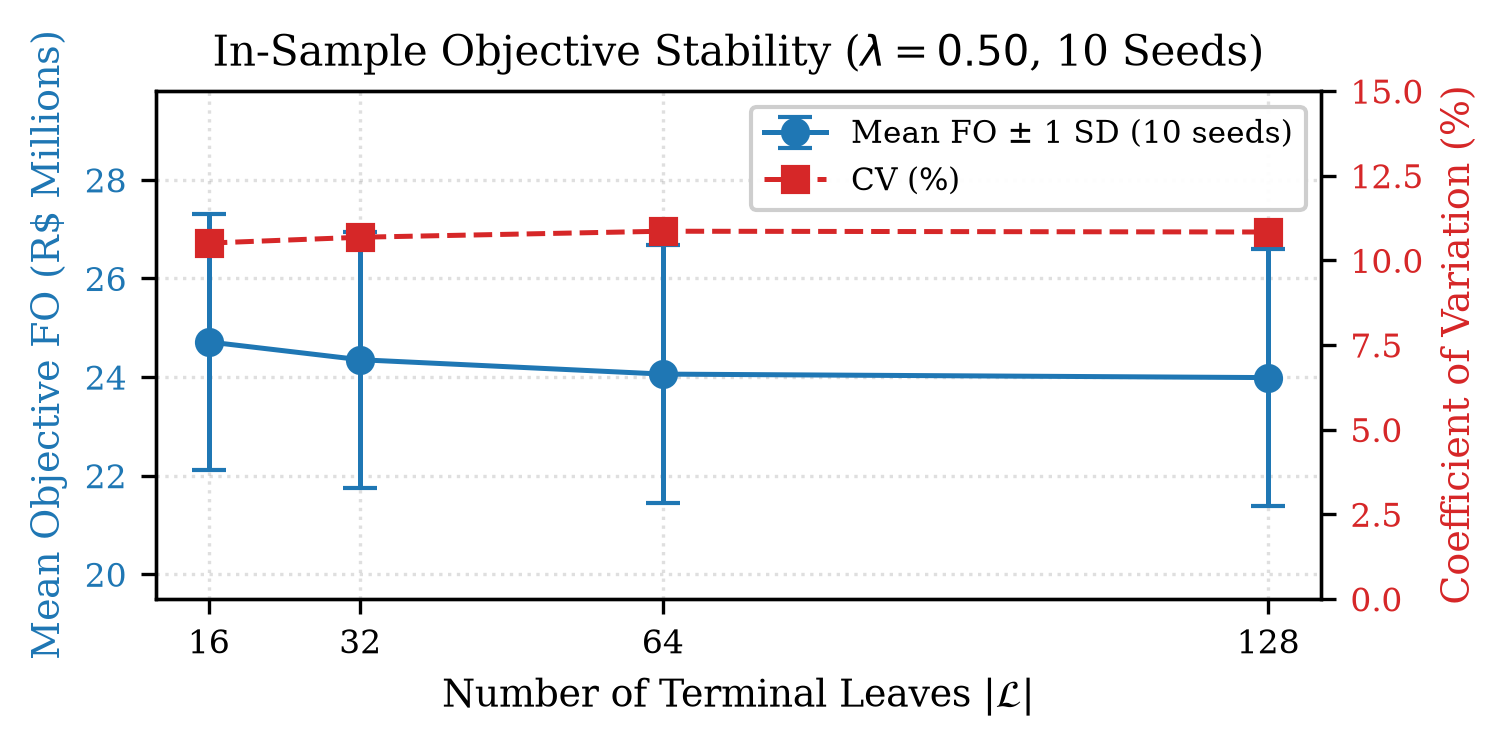
\includegraphics[width=0.92\columnwidth]{fig_tempr_estabilidade.png}
\caption{In-sample scenario tree resolution analysis across 10 independent seeds at $\lambda = 0.50$ ($P^{\text{cli}} = \text{R\$}\,160/\text{MWh}$, $|\mathcal{L}| \in \{16, 32, 64, 128\}$ leaves), showing Mean Objective $\mathrm{FO}$ ($\pm 1$ SD, left axis) and CV (\%, right axis).}
\label{fig:estabilidade}
\end{figure}

\subsection{In-Sample Tree Resolution and Kaut--Wallace Stability}
Across 10 independent seeds at $\lambda = 0.50$ (Fig.~\ref{fig:estabilidade}), Mean $\mathrm{FO}$ decreases monotonically from $\text{R\$}\,24.71\text{M}$ (16 leaves) to $\text{R\$}\,24.35\text{M}$ (32), $\text{R\$}\,24.06\text{M}$ (64), and $\text{R\$}\,23.99\text{M}$ (128 leaves) as finer branching removes upward tail-quantization bias in $\mathrm{CVaR}_{0.05}^{\mathrm{profit}}$ ($\text{R\$}\,23.87\text{M} \to \text{R\$}\,22.51\text{M}$ while $\mathbb{E}[R]$ stays near $\text{R\$}\,25.47\text{M}$). Cross-seed dispersion stays near $\text{SD} \approx \text{R\$}\,2.60\text{M}$ ($\text{CV} = 10.83\%$ relative to the tighter ACL retail margin) at $N = 1,024$ and shrinks to $\text{SD} = \text{R\$}\,1.51\text{M}$ ($\text{CV} = 6.28\%$) at $N = 4,096$ (Supplementary Table~S2). Following Kaut and Wallace~\cite{KautWallace2007} on an $N = 16,384$ reference tree ($\mathrm{FO}_{\text{ref}}(\text{ME-R}) = \text{R\$}\,23.78\text{M}$, Table~S3), out-of-sample dispersion falls to $\text{CV} = 1.37\%$ ($3.01\%$ optimality gap). Evaluating the paired difference $\text{ME-R} - \text{ME}$ out-of-sample on the same $N = 16,384$ reference tree gives $\Delta\mathrm{FO}_{\text{ref}} = +\text{R\$}\,0.45\text{M}$ for the two reference-tree optima and a 10-seed paired OOS gain of $+1.37 \pm 0.74\text{M}$ (95\% CI $[+0.84, +1.90]\text{M}$, positive in 10/10 seeds; $\Delta\mathrm{CVaR}_{\text{OOS}} = +2.86 \pm 1.46\text{M}$), for root decisions from the smaller trees with recourse reoptimized on that reference tree; these are distinct policy comparisons.

\section{Computational Results and Regulatory Backing}
\label{sec:results}

By construction, $\mathrm{FO}(\text{ME-R}) \ge \mathrm{FO}(\text{ME}) \ge \mathrm{FO}(\text{2S}) \ge \mathrm{FO}(\text{HEUR})$ holds in-sample on every tree, with $\text{ME-R} = \text{ME} = \text{2S}$ at $\lambda = 0.0$. Each 128-leaf LP comprises 10,477 continuous variables and 7,676 constraints (0.065\% matrix density, 52.4\,MB peak memory) and solves in $657\,\text{ms}$ on average under HiGHS~1.16.

\subsection{10-Seed Paired In-Sample Efficiency and Classical Metrics}
Because single-seed realizations sit slightly above the multi-seed mean (Seed 2026 $\mathrm{FO} = \text{R\$}\,25.82\text{M}$ vs.\ 10-seed mean $\text{R\$}\,23.99\text{M}$ at $\lambda = 0.50$), Table~\ref{tab:resultados_fundidos} leads with the 10-seed means and paired within-tree differences ($\text{ME-R} - \text{ME}$, $df=9$, $t_{0.975,9}=2.262$; full seven-$\lambda$ Seed-2026 and paired tables appear in Supplementary Tables~S5--S6). For all $\lambda > 0$, resale gains are positive in 10/10 seeds: at $\lambda = 0.50$, $\Delta\mathrm{FO} = +0.92 \pm 0.36\text{M}$ ($+\text{R\$}\,0.75/\text{MWh}$, $+3.98\%$ of ME objective, 95\% CI $[+0.66, +1.17]\text{M}$) and $\Delta\mathrm{CVaR}_{0.05}^{\mathrm{profit}} = +1.96 \pm 0.77\text{M}$ (CI $[+1.41, +2.51]\text{M}$).

\begin{table}[t]
\centering
\caption{10-Seed Mean $\mathrm{FO}$ and Paired Resale Gains ($\text{ME-R} - \text{ME}$, 128 Leaves, $P^{\text{cli}} = \text{R\$}\,160/\text{MWh}$, 95\% $t$-CI).}
\label{tab:resultados_fundidos}
\scriptsize
\setlength{\tabcolsep}{1.2pt}
\begin{tabular}{cccccc}
\toprule
$\lambda$ & ME-R & ME & $\Delta\mathrm{FO}$ & $\Delta\mathrm{FO}$ & $\Delta\mathrm{CVaR}_{0.05}^{\mathrm{profit}}$ \\
 & Mean FO & Mean FO & (R\$ M) [95\% CI] & (R\$/MWh) & (R\$ M) [95\% CI] \\
\midrule
0.00 & 26.53 & 26.53 & $+0.00$ [0.00, 0.00] & $+0.00$ & $+0.00$ [0.00, 0.00] \\
0.10 & 25.26 & 25.14 & $+0.12$ [0.07, 0.16] & $+0.09$ & $+1.57$ [1.10, 2.05] \\
0.30 & 24.58 & 24.08 & $+0.50$ [0.36, 0.64] & $+0.41$ & $+1.96$ [1.39, 2.52] \\
0.50 & 23.99 & 23.07 & $+0.92$ [0.66, 1.17] & $+0.75$ & $+1.96$ [1.41, 2.51] \\
0.70 & 23.40 & 22.06 & $+1.34$ [0.97, 1.71] & $+1.09$ & $+1.97$ [1.43, 2.51] \\
0.90 & 22.82 & 21.06 & $+1.76$ [1.28, 2.24] & $+1.44$ & $+1.97$ [1.43, 2.51] \\
0.95 & 22.68 & 20.81 & $+1.87$ [1.36, 2.38] & $+1.52$ & $+1.97$ [1.43, 2.51] \\
\bottomrule
\end{tabular}
\end{table}

\begin{figure}[t]
\centering
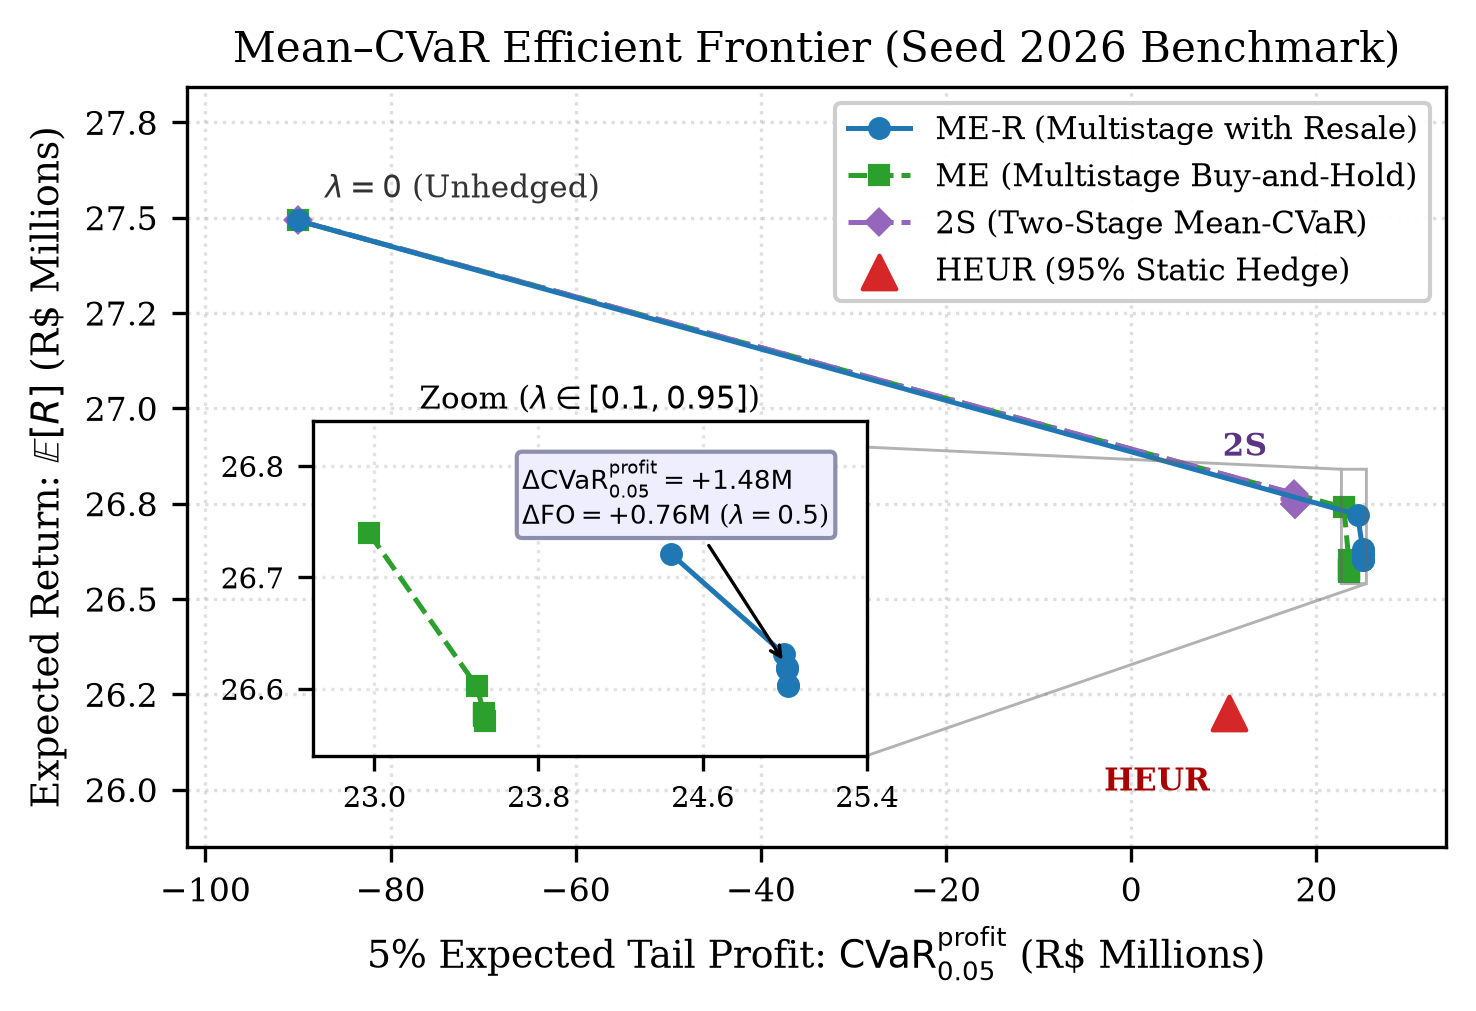
\includegraphics[width=0.90\columnwidth]{fig_tempr_fronteira.png}
\caption{Illustrative Seed-2026 Mean--CVaR efficient frontier in the $(\mathrm{CVaR}_{0.05}^{\mathrm{profit}}, \mathbb{E}[R])$ plane comparing ME-R, ME, 2S, and HEUR ($P^{\text{cli}} = \text{R\$}\,160/\text{MWh}$); the inset zooms into $\lambda \in [0.10, 0.95]$.}
\label{fig:fronteira}
\end{figure}

Fig.~\ref{fig:fronteira} illustrates the efficient frontier on Seed~2026 alongside the two-stage benchmark (2S) and static HEUR. Moving from $\lambda = 0$ (where $q^* = 0$ yields $\mathrm{CVaR}_{0.05}^{\mathrm{profit}} = -\text{R\$}\,90.04\text{M}$) to $\lambda = 0.10$ lifts tail profit above $\text{R\$}\,24.4\text{M}$ at under $\text{R\$}\,0.77\text{M}$ expected profit cost. Table~\ref{tab:vss_evpi} decomposes classical stochastic metrics~\cite{BirgeLouveaux2011} on Seed~2026: at $\lambda = 0.0$, Wait-and-See ($\text{WS} = 36.65\text{M}$) exceeds the Recourse Problem ($\text{RP} = 27.49\text{M}$) and Expected Value of the Expected Value solution ($\text{EEV} = 27.49\text{M}$), yielding Expected Value of Perfect Information $\text{EVPI} = \text{R\$}\,9.16\text{M}$ ($+33.33\%$) and canonical Value of the Stochastic Solution $\text{VSS} = 0.00\text{M}$ by construction since $q^* = 0$ on the expected scenario. At $\lambda = 0.50$, sequential recourse raises $\mathrm{VMR}$ over two-stage 2S ($\text{FO}_{\text{2S}} = 22.23\text{M}$) by $+\text{R\$}\,2.83\text{M}$ for buy-and-hold ME ($25.06\text{M}$) and $+\text{R\$}\,3.59\text{M}$ for ME-R ($25.82\text{M}$, adding $+\text{R\$}\,0.76\text{M}$ from resale).

\begin{table}[t]
\centering
\caption{Seed-2026 Stochastic Metrics ($\lambda=0.0$), Two-Stage Benchmark, and Value of Multistage Recourse ($\lambda=0.50$, R\$ Millions).}
\label{tab:vss_evpi}
\scriptsize
\setlength{\tabcolsep}{3pt}
\begin{tabular}{lc}
\toprule
Metric & Value (R\$ M) \\
\midrule
$\text{RP} = \text{EEV}$ / $\text{WS}$ ($\lambda = 0.0$) & 27.49 / 36.65 \\
Canonical $\text{VSS}$ / $\text{EVPI}$ ($\lambda = 0.0$) & 0.00 / +9.16 \\
\midrule
Multistage with Resale ($\text{FO}_{\text{ME-R}}$, $\lambda=0.50$) & 25.82 \\
Multistage Buy-and-Hold ($\text{FO}_{\text{ME}}$, $\lambda=0.50$) & 25.06 \\
Two-Stage Mean--CVaR ($\text{FO}_{\text{2S}}$, $\lambda=0.50$) & 22.23 \\
$\mathrm{VMR}_{\text{ME}}$ / $\mathrm{VMR}_{\text{ME-R}}$ ($\text{FO} - \text{FO}_{\text{2S}}$) & +2.83 / +3.59 \\
Unhedged / Zero-Hedge Portfolio ($\lambda=0.50$) & $-31.28$ \\
\bottomrule
\end{tabular}
\end{table}

\subsection{Decree 5.163/2004 Backing Penalties and Coverage Floors}
\label{sec:reg_exp}
Table~\ref{tab:regulatorio} evaluates all strategies across 10 seeds ($\lambda = 0.50$) under three regulatory regimes: \textit{R0} (unconstrained baseline with ex-post audit), \textit{R1} (Decree~5.163/2004 trailing 12-month VR penalty $\pi_{\text{VR}} = \text{R\$}\,231.47/\text{MWh}$ inside the optimization), and \textit{R2} (100\% prudential coverage floor $\underline{c} = 1.0$ plus VR penalty).

\begin{table}[t]
\centering
\caption{10-Seed Regulatory Backing and Coverage-Floor Comparison ($\lambda = 0.50$, $P^{\text{cli}} = \text{R\$}\,160/\text{MWh}$).}
\label{tab:regulatorio}
\scriptsize
\setlength{\tabcolsep}{1.5pt}
\begin{tabular}{lccccc}
\toprule
Regime / & Mean FO & $\mathrm{CVaR}_{0.05}^{\mathrm{profit}}$ & 12M Def. & VR Fine & Gar95 \\
Strategy & (R\$ M / R\$\,MWh$^{-1}$) & (R\$ M) & (GWh) & (R\$ M / Br.\%) & (R\$ M) \\
\midrule
\multicolumn{6}{l}{\textbf{R0: Unconstrained (Ex-Post Regulatory Audit)}} \\
ME-R          & 23.99 / 19.56 & 22.51 & 68.8 & 15.92 / 95.9\% & 19.16 \\
ME            & 23.07 / 18.81 & 20.55 & 45.9 & 10.63 / 83.0\% & 11.59 \\
2S            & 21.31 / 17.38 & 16.93 & 63.6 & 14.73 / 98.7\% & 13.51 \\
HEUR\_95      & 17.86 / 14.56 & 10.49 & 35.2 & 8.15 / 60.9\%  & 10.43 \\
Unhedged      & $-30.92$ / $-25.21$ & $-88.36$ & 510.8 & 118.24 / 100.0\% & 67.91 \\
\midrule
\multicolumn{6}{l}{\textbf{R1: Decree 5.163/2004 + REN 1.090/2024 ($\pi_{\text{VR}} = \text{R\$}\,231.47/\text{MWh}$)}} \\
ME-R          & 23.85 / 19.45 & 22.31 & 0.02 & 0.004 / 3.5\%  & 13.08 \\
ME            & 23.01 / 18.77 & 20.49 & 0.00 & 0.001 / 0.8\%  & 10.70 \\
2S            & 19.93 / 16.25 & 14.71 & 1.76 & 0.41 / 35.5\%  & 12.87 \\
HEUR\_95      & 4.19 / 3.41   & $-8.69$ & 35.2 & 8.15 / 60.9\%  & 10.43 \\
Unhedged      & $-152.99$ / $-124.75$ & $-214.27$ & 510.8 & 118.24 / 100.0\% & 67.91 \\
\midrule
\multicolumn{6}{l}{\textbf{R2: 100\% Prudential Coverage Floor ($\underline{c}=1.0$) + VR Penalty}} \\
ME-R          & 21.35 / 17.41 & 17.16 & 0.00 & 0.000 / 0.3\%  & 10.00 \\
ME            & 20.91 / 17.05 & 16.20 & 0.00 & 0.000 / 0.0\%  & 10.00 \\
2S            & 19.56 / 15.95 & 13.88 & 1.55 & 0.36 / 25.9\%  & 10.00 \\
HEUR\_100     & 10.79 / 8.80  & 1.56  & 22.2 & 5.13 / 53.1\%  & 10.00 \\
\bottomrule
\end{tabular}
\end{table}

Table~\ref{tab:regulatorio} shows regulatory differences that remain hidden in unconstrained models. Under R0, optimal commercializers carry partial spot exposure ($45.9$--$68.8\,\text{GWh}$ trailing deficit) when forwards incur spreads. Once Decree~5.163/2004 VR penalties are enforced (R1), ME-R and ME eliminate almost all backing breaches ($96.5\%$--$99.2\%$ compliance, VR fines $\le \text{R\$}\,0.004\text{M}$) at minimal objective loss ($\text{R\$}\,0.06$--$0.14\text{M}$), while preserving a statistically significant paired resale gain of $+0.84 \pm 0.31\text{M}$ (10/10 seeds) and reducing peak 2-month short collateral exposure ($\text{Gar95}$) from $\text{R\$}\,19.16\text{M}$ to $\text{R\$}\,13.08\text{M}$. Conversely, passive HEUR\_95 declines to $\text{FO} = \text{R\$}\,4.19\text{M}$ ($\mathrm{CVaR} = -\text{R\$}\,8.69\text{M}$) due to $35.2\,\text{GWh}$ deficits ($60.9\%$ breach, $\text{R\$}\,8.15\text{M}$ VR fine), and Unhedged suffers $-\text{R\$}\,152.99\text{M}$ ($\text{R\$}\,118.24\text{M}$ VR fine, $\text{Gar95} = \text{R\$}\,67.91\text{M}$). Imposing a hard 100\% coverage floor (R2) cuts ME-R resale value roughly in half ($+0.44 \pm 0.36\text{M}$, 10/10 seeds) and caps collateral at $\text{R\$}\,10.00\text{M}$, while even static HEUR\_100 still incurs $53.1\%$ breach incidence ($\text{R\$}\,5.13\text{M}$ fine) under positive demand churn.

\section{Out-of-Sample Backtesting Against Exogenous Curves}
\label{sec:backtest}

\subsection{20-Seed Historical Rolling Backtest (2024--2025)}
The scenario tree supplies internally consistent prices for optimization, while exogenous execution quotes assess decisions against a common market rather than their own forecasts. All forward executions in the 2024--2025 expanding-window rolling backtest ($s_0 \in \{2024, \dots, 2043\}$, 17,544 unobserved hours) settle against an exogenous market forward curve estimated without look-ahead up to month $3q-1$: a seasonal log-AR(1) model with Bayesian calendar-month shrinkage, $\ln \text{PLD}_{s,t} = \hat{\mu}_{s,m(t)} + r_{s,t}$, $r_{s,t} = \hat{\phi}_s r_{s,t-1} + \epsilon_{s,t}$, clipped to ANEEL bounds ($\text{Q0}$ mean SE forward $\text{R\$}\,115.74/\text{MWh}$, vs.\ $\text{R\$}\,122.86/\text{MWh}$ on the base tree). We also evaluate two hybrid policies initialized with HEUR's 95\% root hedge: \textit{HEUR+R (resale-only)}, permitting only $x^- \ge 0$ for $q \ge 1$, and \textit{HEUR+R (full)}, permitting purchases and resales for $q \ge 1$.

\begin{table}[t]
\centering
\caption{20-Seed Rolling Backtest (2024--2025, $P^{\text{cli}} = \text{R\$}\,160/\text{MWh}$, Exogenous AR(1) Forward Curve, Mean $\pm$ Seed SD).}
\label{tab:backtest_20seeds}
\scriptsize
\setlength{\tabcolsep}{1.5pt}
\begin{tabular}{@{}lccccc@{}}
\toprule
Strategy & Profit (R\$ M) & Worst & Cash & 12M Def. / & GarPeak \\
 & [R\$\,MWh$^{-1}$] & Mo. & Min & VR Fine & (R\$ M) \\
\midrule
ME            & $49.57\!\pm\!6.38$ [40.4] & $-1.36$ & $-29.30$ & 4.4 / 1.02   & 6.95 \\
ME-R          & $43.02\!\pm\!8.81$ [35.0] & $-4.83$ & $-31.35$ & 58.7 / 13.58 & 12.57 \\
HEUR+R (full) & $38.65\!\pm\!5.06$ [31.5] & $-2.78$ & $-36.47$ & 23.6 / 5.45  & 8.56 \\
HEUR          & $37.23\!\pm\!0.00$ [30.3] & $-1.01$ & $-36.47$ & 25.7 / 5.95  & 6.17 \\
HEUR+R (res.) & $30.92\!\pm\!9.30$ [25.2] & $-6.65$ & $-36.47$ & 84.5 / 19.56 & 16.68 \\
Unhedged      & $-28.35\!\pm\!0.00$ [$-23.1$] & $-17.03$ & $-17.03$ & 514.1 / 118.99 & 39.16 \\
\bottomrule
\end{tabular}
\end{table}

\begin{figure}[t]
\centering
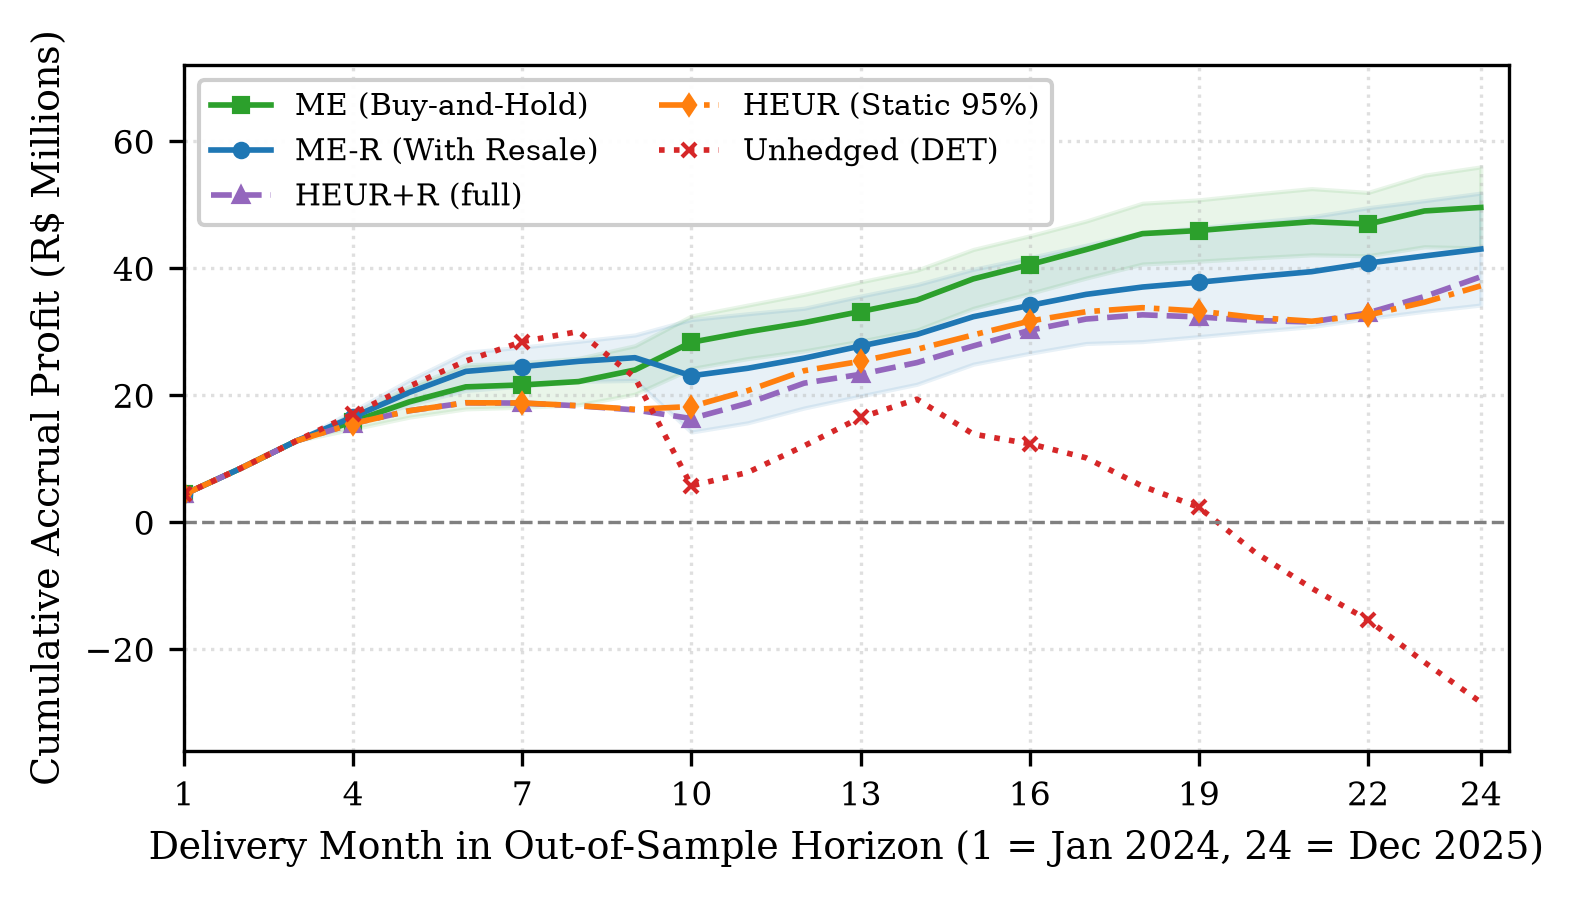
\includegraphics[width=\columnwidth]{fig_tempr_backtest.png}
\caption{20-seed mean cumulative accrual profit across 2024--2025 under the exogenous seasonal log-AR(1) market forward curve (shaded bands show $\pm 1$ seed SD for ME and ME-R).}
\label{fig:backtest}
\end{figure}

Table~\ref{tab:backtest_20seeds} and Fig.~\ref{fig:backtest} summarize out-of-sample performance once own-tree forward execution is removed:
\begin{enumerate}
    \item \textit{Insignificant Mean Difference Between Resale and Buy-and-Hold, Paired with Lower Risk for Buy-and-Hold:} Without demand churn (historical load stays flat at $D^{\text{base}}$), buy-and-hold ME ($\text{R\$}\,49.57\text{M}$, $\text{R\$}\,40.36/\text{MWh}$) finishes ahead of ME-R ($\text{R\$}\,43.02\text{M}$) in 16/20 seeds ($-\text{R\$}\,6.56 \pm 9.64\text{M}$ total, or $-\text{R\$}\,0.273\text{M}$/mo. on average), yet the moving-block bootstrap 95\% CI ($[-1.102, +0.325]\,\text{M}$/mo.) includes zero, so the mean profit difference is not statistically significant. Rather, the clearest separation appears in risk and regulatory metrics: ME exhibits lower cross-seed dispersion ($\text{SD}\;\text{R\$}\,6.38\text{M}$ vs.\ $\text{R\$}\,8.81\text{M}$), milder worst-month and monthly tail losses ($-\text{R\$}\,1.36\text{M}$ vs.\ $-\text{R\$}\,4.83\text{M}$; monthly $\mathrm{CVaR}_{0.05}^{\mathrm{profit}}\;-\text{R\$}\,0.76\text{M}$ vs.\ $-\text{R\$}\,2.64\text{M}$), smaller trailing 12-month backing deficits ($4.4$ vs.\ $58.7\,\text{GWh}$; $\text{R\$}\,1.02\text{M}$ vs.\ $\text{R\$}\,13.58\text{M}$ implied VR fine), and lower peak 2-month collateral ($\text{R\$}\,6.95\text{M}$ vs.\ $\text{R\$}\,12.57\text{M}$). When 2024--2025 spot prices rallied above tree expectations, ME-R unwound inherited forwards at lower exogenous AR(1) quotes, whereas ME retained its cover; ME also exceeds passive HEUR ($\text{R\$}\,37.23\text{M}$) in 20/20 seeds ($+\text{R\$}\,12.34\text{M}$, bootstrap CI $[+0.010, +1.141]\,\text{M}$/mo.).
    \item \textit{Hybrid HEUR+R Tradeoffs:} Similarly, HEUR+R (resale-only) loses $-\text{R\$}\,6.31\text{M}$ relative to HEUR ($0/20$ wins) by selling off cheap initial hedges, whereas HEUR+R (full) adds $+\text{R\$}\,1.42\text{M}$ over HEUR ($14/20$ seeds, CI $[-0.191, +0.243]\,\text{M}$/mo.) while trailing ME by $-\text{R\$}\,10.92\text{M}$.
    \item \textit{Hedging Value Over Unhedged:} All hedged policies substantially outperform Unhedged ($-\text{R\$}\,28.35\text{M}$, $514.1\,\text{GWh}$ backing deficit, $\text{R\$}\,118.99\text{M}$ implied VR fine, $\text{GarPeak} = \text{R\$}\,39.16\text{M}$).
\end{enumerate}

\subsection{1,000-Trajectory Independent Synthetic OOS Simulation}
To achieve high statistical power under realistic demand churn, we simulate 1,000 24-month trajectories from an independent non-Markovian data-generating process (DGP) combining circular stationary block bootstrap~\cite{PolitisRomano1994} (mean block 3 months) with quarterly regime-jump multipliers (probability 0.12) and AR(1) retail demand ($\rho_{\text{AR}} = 0.75$, $\eta \sim \mathcal{N}(0, 0.055^2)$, clipped to $[0.75, 1.25]$), rolling with seed $2026 + 17q$. Every strategy executes against the exact analytical conditional expectation of the DGP given the last realized pool state at $3q-1$. In this synthetic setting, mean-profit differences principally reflect trading spreads and sampling noise, rather than a systematic forward risk premium. Panel~A evaluates the disjoint pre-test DGP pool (2021--2023) with the sparse 2021--2023 tree; Panel~B evaluates the same disjoint DGP with the IPCA-deflated diversified 2001--2023 tree; and Panel~C tests sensitivity to sampling the full 60-month 2021--2025 DGP pool.

\begin{table}[t]
\centering
\caption{Out-of-Sample Performance Across 1,000 Independent Synthetic Paths (R\$ M, Exact Exogenous DGP Forward Curve).}
\label{tab:oos_sintetico}
\scriptsize
\setlength{\tabcolsep}{0.2pt}
\begin{tabular}{@{}lcccc@{}}
\toprule
Strategy & Mean (SD) & Traj. & $\Delta$ vs.\ ME-R [95\% CI] & 12M Def. / \\
 & (R\$ M) & CVaR & (Win \% vs.\ ME-R) & Gar95 \\
\midrule
\multicolumn{5}{@{}l}{\textbf{Panel A: Disjoint 2021--2023 DGP + Sparse 2021--2023 Tree}} \\
ME-R          & 4.72 (30.31) & $-82.63$ & Baseline & 67.4 / 62.4 \\
ME            & 4.26 (27.38) & $-74.45$ & $-0.46\,[-1.24,+0.32]$ (38.2\%) & 17.5 / 61.8 \\
HEUR          & 3.63 (19.08) & $-50.93$ & $-1.09\,[-2.30,+0.11]$ (31.6\%) & 27.9 / 57.4 \\
HEUR+R (res)  & 3.24 (25.29) & $-72.49$ & $-1.48$ (--) & 89.9 / 59.9 \\
HEUR+R (all)  & 3.28 (21.55) & $-59.45$ & $-1.44\,[-2.54,-0.34]$ (29.0\%) & 38.1 / 57.9 \\
Unhedged      & 5.95 (60.07) & $-140.19$ & $+1.23$ (--) & 513.3 / 70.3 \\
\midrule
\multicolumn{5}{@{}l}{\textbf{Panel B: Disjoint 2021--2023 DGP + IPCA 2001--2023 Tree}} \\
ME-R          & 3.63 (18.74) & $-51.15$ & Baseline & 6.5 / 57.4 \\
ME            & 3.81 (19.65) & $-53.42$ & $+0.18\,[-0.26,+0.61]$ (39.0\%) & 0.1 / 57.4 \\
HEUR          & 3.63 (19.08) & $-50.93$ & $-0.00\,[-0.45,+0.45]$ (59.1\%) & 27.9 / 57.4 \\
HEUR+R (res)  & 3.65 (19.14) & $-51.04$ & $+0.02$ (--) & 29.2 / 57.4 \\
HEUR+R (all)  & 3.45 (19.24) & $-52.52$ & $-0.18\,[-0.50,+0.13]$ (57.4\%) & 18.1 / 57.4 \\
Unhedged      & 5.95 (60.07) & $-140.19$ & $+2.32$ (--) & 513.3 / 70.3 \\
\midrule
\multicolumn{5}{@{}l}{\textbf{Panel C: Full 2021--2025 DGP + Sparse 2021--2023 Tree}} \\
ME-R          & $-11.88$ (27.34) & $-82.58$ & Baseline & 69.7 / 58.5 \\
ME            & $-11.04$ (24.09) & $-73.85$ & $+0.83\,[+0.08,+1.58]$ (45.6\%) & 23.3 / 57.3 \\
HEUR          & $-11.94$ (16.68) & $-58.86$ & $-0.06\,[-1.19,+1.07]$ (42.0\%) & 27.7 / 45.9 \\
HEUR+R (res)  & $-12.89$ (22.38) & $-77.48$ & $-1.01$ (--) & 100.7 / 55.0 \\
HEUR+R (all)  & $-12.80$ (19.75) & $-69.39$ & $-0.92\,[-1.96,+0.11]$ (38.0\%) & 39.7 / 49.7 \\
Unhedged      & $-10.42$ (54.37) & $-136.42$ & $+1.45$ (--) & 513.7 / 66.4 \\
\bottomrule
\end{tabular}
\end{table}

Table~\ref{tab:oos_sintetico} summarizes three findings across 1,000 independent churn trajectories:
\begin{enumerate}
    \item \textit{Sparse 2021--2023 Calibration (Panel~A):} On the disjoint pre-test DGP, ME-R ($4.72\text{M}$) delivers a statistically insignificant $+0.46\text{M}$ mean difference over ME ($95\%$ CI $[-0.32, +1.24]\text{M}$, $61.8\%$ path win rate) and $+1.09\text{M}$ over HEUR ($[-0.11, +2.30]\text{M}$, $68.4\%$), while incurring deeper tail losses ($\mathrm{CVaR}_{0.05}^{\mathrm{profit}} = -82.63\text{M}$ vs.\ $-74.45\text{M}$ for ME and $-50.93\text{M}$ for HEUR) and larger 12-month backing deficits ($67.4$ vs.\ $17.5\,\text{GWh}$). Both hybrid HEUR+R policies trail static HEUR, and Unhedged carries extreme tail risk ($-140.19\text{M}$) and $513.3\,\text{GWh}$ backing deficits.
    \item \textit{IPCA-Deflated 2001--2023 Calibration (Panel~B):} Populating every seasonal regime cell via IPCA-deflated 2001--2023 sampling substantially improves multistage tail resilience and regulatory compliance under exogenous curves: ME-R and ME improve trajectory CVaR to $-51.15\text{M}$ and $-53.42\text{M}$ (matching HEUR's $-50.93\text{M}$) and cut 12-month deficits to $6.5$ and $0.1\,\text{GWh}$ (vs.\ $27.9\,\text{GWh}$ for HEUR), while halving profit variance ($\text{SD} \approx 19\text{M}$). However, mean profit differences vanish: ME ($3.81\text{M}$) slightly leads ME-R ($3.63\text{M}$, CI $[-0.26, +0.61]\text{M}$) and ME-R matches HEUR ($+0.00\text{M}$, CI $[-0.45, +0.45]\text{M}$).
    \item \textit{2021--2025 Structural Shift Sensitivity (Panel~C):} Drawing DGP blocks from the full 2021--2025 pool shifts mean profits negative ($\approx -11\text{M}$ to $-12\text{M}$) at fixed $P^{\text{cli}} = \text{R\$}\,160/\text{MWh}$, reflecting margin compression when unindexed retail tariffs face sustained spot escalation. Under this drift, buy-and-hold ME ($-11.04\text{M}$) has a higher mean than ME-R ($-11.88\text{M}$) by $+0.83\text{M}$ (CI $[+0.08, +1.58]\text{M}$), despite winning on only $45.6\%$ of paths, while passive HEUR retains the best tail protection ($\mathrm{CVaR} = -58.86\text{M}$) and lowest collateral ($\text{Gar95} = 45.88\text{M}$).
\end{enumerate}

\section{Sensitivity Analyses and Structural Extensions}
\label{sec:sens}

\subsection{Systemic Reserve Charges, Spreads, Demand Volatility, and Tariff}
Table~\ref{tab:sensibilidade} shows Seed-2026 sensitivities at $\lambda = 0.50$ ($P^{\text{cli}} = \text{R\$}\,160/\text{MWh}$). Because deterministic $\tau_{\text{reg}}$ multiplies exogenous expected load ($1,221.4\,\text{GWh}$), each $\text{R\$}\,15.00/\text{MWh}$ increment shifts $\mathbb{E}[R]$, $\mathrm{CVaR}_{0.05}^{\mathrm{profit}}$, and $\mathrm{FO}$ linearly by $-\text{R\$}\,18.32\text{M}$ without altering contracting decisions. Narrowing half-spread $\sigma$ from $1.0\%$ to $0.5\%$ raises $\mathrm{FO}(\text{ME-R})$ by $+\text{R\$}\,0.44\text{M}$ ($\text{R\$}\,26.26\text{M}$), whereas widening $\sigma$ to $3.0\%$ lowers $\mathrm{FO}$ to $\text{R\$}\,24.08\text{M}$ ($-\text{R\$}\,1.74\text{M}$). Increasing demand churn volatility $\sigma_D$ from $0.08$ to $0.25$ at $\sigma = 1.0\%$ raises $\Delta\mathrm{CVaR}_{0.05}^{\mathrm{profit}}$ from $+\text{R\$}\,1.48\text{M}$ ($116.2\,\text{GWh}$ resold, $9.5\%$ of demand) to $+\text{R\$}\,5.53\text{M}$ ($292.6\,\text{GWh}$, $25.2\%$). Compressing $\sigma$ to $0.2\%$ expands resale volume to $187.1\,\text{GWh}$ ($\sigma_D=0.08$) and $353.9\,\text{GWh}$ ($\sigma_D=0.25$). Varying $P^{\text{cli}} \in [150, 260]\,\text{R\$/MWh}$ (Table~S10) keeps absolute resale gains stable at $\text{R\$}\,0.76$--$1.05\text{M}$ ($\text{R\$}\,0.62$--$0.86/\text{MWh}$), while scaling relative objective share from $0.72\%$ ($P^{\text{cli}} = 260$) to $6.76\%$ ($P^{\text{cli}} = 150$).

\begin{table}[t]
\centering
\caption{Impact of ESS/EER Charges and Forward Half-Spreads ($\lambda = 0.50$, Seed 2026, $P^{\text{cli}} = \text{R\$}\,160/\text{MWh}$).}
\label{tab:sensibilidade}
\scriptsize
\setlength{\tabcolsep}{4pt}
\begin{tabular}{ccccc}
\toprule
$\tau_{\text{reg}}$ & Half-Spread & $\mathbb{E}[R]$ & $\mathrm{CVaR}_{0.05}^{\mathrm{profit}}$ & Obj.\ (FO) \\
(R\$/MWh) & ($\sigma$) & (R\$ M) & (R\$ M) & (R\$ M) \\
\midrule
0.0  & 1.0\% & 44.97 & 43.11 & 44.04 \\
15.0 & 1.0\% & 26.62 & 25.01 & 25.82 \\
30.0 & 1.0\% & 8.22  & 6.82  & 7.52  \\
\midrule
15.0 & 0.5\% & 27.04 & 25.47 & 26.26 \\
15.0 & 1.5\% & 26.19 & 24.56 & 25.38 \\
15.0 & 3.0\% & 24.93 & 23.22 & 24.08 \\
\bottomrule
\end{tabular}
\end{table}

\subsection{Forward Risk Premia: Constant vs.\ Maturity-Decaying Curves}
\label{sec:premio}
Table~\ref{tab:premio_risco} compares constant risk premia ($\psi_0$) against a maturity-decaying term structure ($\psi_0 \tau_{\nu,k,p}$) at $\lambda = 0.50$ (full $\lambda \in \{0.0, 0.5\}$ results in Table~S12). At $\lambda = 0.0$ and constant $\psi_0 < 0$, iterated expectations create timing indifference between $t=0$ and $t \ge 1$ ($q_0^{\text{SE}} = 8.04\,\text{MWmed}$), which maturity decay breaks ($q_0^{\text{SE}} = 50.61$--$53.28\,\text{MWmed}$). At $\lambda = 0.50$ and $\psi_0 \in \{+5\%, +10\%\}$, constant premia inflate $\Delta\mathrm{FO}$ to $+\text{R\$}\,4.35\text{M}$ and $+\text{R\$}\,8.89\text{M}$ via spread-arbitrage premium harvesting ($837.1$--$920.1\,\text{GWh}$ resold); maturity-decaying premia reduce resale turnover ($346.4$--$495.6\,\text{GWh}$) and capture only hedge-unwind gains of $+\text{R\$}\,1.29\text{M}$ and $+\text{R\$}\,2.33\text{M}$.

\begin{table}[t]
\centering
\caption{Constant vs.\ Maturity-Decaying Forward Risk Premia ($\lambda = 0.50$, Seed 2026; FO in R\$ M, $q_0^{\text{SE}}$ in MWmed).}
\label{tab:premio_risco}
\scriptsize
\setlength{\tabcolsep}{2.5pt}
\begin{tabular}{ccccccc}
\toprule
$\psi_0$ & Curve & ME-R & ME & HEUR & $\Delta\mathrm{FO}$ & $q_0^{\text{SE}}$ \\
\midrule
$-10\%$ & Const. & 41.27 & 40.58 & 31.41 & +0.69 & 41.40 \\
$-5\%$  & Const. & 33.40 & 32.69 & 24.88 & +0.71 & 42.28 \\
$0\%$   & --     & 25.82 & 25.06 & 18.36 & +0.76 & 48.10 \\
$+5\%$  & Const. & 23.50 & 19.16 & 11.83 & +4.35 & 46.04 \\
$+10\%$ & Const. & 22.45 & 13.56 & 5.31  & +8.89 & 47.92 \\
\midrule
$+5\%$  & Decay  & 23.37 & 22.09 & 14.97 & +1.29 & 23.67 \\
$+10\%$ & Decay  & 21.53 & 19.20 & 11.59 & +2.33 & 26.37 \\
\bottomrule
\end{tabular}
\end{table}

\subsection{Structural Extensions: Hourly Modulation and FTR Proof-of-Concept}
\label{sec:ext_res}
For Extension~1 (hourly modulation, Table~S8), stylized 24-hour archetypes evaluated over the 26,280-hour training and 17,544-hour test series show that because $\gamma_{s,m}$ acts as an exogenous pass-through on demand, reoptimizing flat monthly forwards yields modest in-sample gains ($+\text{R\$}\,0.10\text{M}$ to $+\text{R\$}\,0.54\text{M}$), whereas 2024--2025 midday solar depression and evening ramps shift ex-post profit by $+\text{R\$}\,7.42\text{M}$ (industrial) and $+\text{R\$}\,9.21\text{M}$ (commercial) vs.\ $-\text{R\$}\,8.11\text{M}$ (residential). For Extension~2 ($\text{NE}\to\text{SE}$ FTRs, Table~S9), risk-averse retailers hold near-zero cross-submarket contracts without FTRs ($0.24\,\text{GWh}$); a frictionless monthly FTR ($c_{\text{FTR}} = 0$) shifts $650.36\,\text{GWh}$ cross-submarket ($526.84\,\text{GWh}$ FTR) for only $+\text{R\$}\,0.007\text{M}$ ($+0.026\%$), dropping to $0.00\,\text{GWh}$ at $c_{\text{FTR}} \ge \text{R\$}\,1.00/\text{MWh}$, while Jensen's inequality leaves hourly congestion option value ($\text{R\$}\,4.48$ and $\text{R\$}\,28.36/\text{MWh}$) above monthly spread averages ($\text{R\$}\,3.70$ and $\text{R\$}\,28.20/\text{MWh}$).

\section{Conclusion and Policy Implications}
\label{sec:conclusion}

Across paired scenario trees incorporating joint price--demand branching and realistic ACL retail margins ($P^{\text{cli}} = \text{R\$}\,160/\text{MWh}$), backed forward resale consistently enhances in-sample portfolio efficiency ($+0.92 \pm 0.36\text{M}$, $\text{R\$}\,0.75/\text{MWh}$, 10/10 seeds at $\lambda = 0.50$; $+\text{R\$}\,1.37 \pm 0.74\text{M}$ on a 16,384-path Kaut--Wallace reference tree; and $\mathrm{VMR} = +\text{R\$}\,3.59\text{M}$ over two-stage optimization). Enforcing Decree~5.163/2004 and ANEEL REN~1.090/2024 trailing 12-month backing penalties also illustrates the practical value of dynamic multistage recourse: ME-R and ME achieve $96.5\%$--$99.2\%$ regulatory compliance and limit 2-month short collateral calls, whereas passive 95\% hedging suffers $60.9\%$ breach incidence ($\text{R\$}\,8.15\text{M}$ VR penalty) and unhedged portfolios incur $-\text{R\$}\,152.99\text{M}$ penalized objective.

Out-of-sample evaluation against exogenous market forward curves shows clear limits to dynamic resale. On flat 2024--2025 historical load under a seasonal log-AR(1) market forward curve, the mean profit difference between rolling ME-R and buy-and-hold ME ($-\text{R\$}\,0.273\,\text{M}$/mo., 95\% bootstrap CI $[-1.102, +0.325]\,\text{M}$/mo.) is statistically insignificant despite ME finishing ahead in 16/20 seeds; the substantive advantage of buy-and-hold lies in risk and regulatory metrics, namely lower cross-seed dispersion ($6.38\text{M}$ vs.\ $8.81\text{M}$), smaller monthly tail losses ($-0.76\text{M}$ vs.\ $-2.64\text{M}$ CVaR), lower trailing 12-month deficits ($4.4$ vs.\ $58.7\,\text{GWh}$), and lower peak collateral ($6.95\text{M}$ vs.\ $12.57\text{M}$), alongside significant gains over static HEUR ($+\text{R\$}\,12.34\,\text{M}$, $20/20$ seeds, CI $[+0.010, +1.141]\,\text{M}$/mo.). Across 1,000 independent synthetic churn trajectories evaluated at exact DGP forward curves, resale adds an insignificant $+0.46\text{M}$ (CI $[-0.32, +1.24]\text{M}$) under sparse 2021--2023 trees while trailing buy-and-hold ME and static HEUR in trajectory CVaR ($-82.63\text{M}$ vs.\ $-74.45\text{M}$ and $-50.93\text{M}$). Diversifying the scenario tree via IPCA-deflated 2001--2023 sampling cuts multistage tail losses to $-51.15\text{M}$ and shrinks 12-month backing deficits to $6.5\,\text{GWh}$ (ME-R) and $0.1\,\text{GWh}$ (ME), yet leaves mean profits statistically indistinguishable across ME-R, ME, and HEUR. When 2021--2025 spot shifts enter the DGP, buy-and-hold ME has a higher mean than ME-R ($+0.83\text{M}$, CI $[+0.08, +1.58]\text{M}$), winning $45.6\%$ of paths. Scenario-tree misspecification, multi-decade inflation calibration, and market forward divergence, rather than secondary trading constraints alone, therefore govern real-world dynamic hedging performance.

For market venues and clearinghouses (BBCE and B3), narrowing bid-ask spreads from $1.0\%$ to $0.2\%$ expands secondary turnover from $116.2$ to $187.1\,\text{GWh}$ ($\sigma_D = 0.08$) and up to $353.9\,\text{GWh}$ under higher churn ($\sigma_D = 0.25$). For regulators overseeing Type~1 retail marketers, the in-sample R1 comparison suggests that enforcing the 2025 VR of $\text{R\$}\,231.47/\text{MWh}$ entails smaller objective and liquidity costs than the R2 coverage floor. This policy comparison rests on in-sample results and does not establish an out-of-sample effect on systemic default risk. Future work will incorporate retail contract volume flexibility bands, stochastic ESS/EER levies coupled to hydrology, and hourly-settled FTR valuation.

\section*{Data and Code Availability}
Historical CCEE spot prices are available at \url{https://www.ccee.org.br}. Reproducible optimization models, scenario builders, backtesting scripts, and figure code are publicly available at \url{https://github.com/glaubosclimaco/contract-resale-acl} (tag v1.0-tempr-submission), and will be archived with a Zenodo DOI upon acceptance.

\bibliographystyle{IEEEtran}
\bibliography{refs}

\end{document}
